\chapter{Factory Method模式}
\section{工厂方法模式的概念}
\textbf{工厂方法(FactoryMethod)模式的定义:}定义一个创建产品对象的工厂接口,将产品对象的实际创建工作推迟到具体子工厂类当中。这满足创建型模式中所要求的“创建与使用相分离”的特点。
\par 我们把被创建的对象称为“产品”,把创建产品的对象称为“工厂”。如果要创建的产品不多,只要一个工厂类就可以完成,这种模式叫“简单工厂模式”,它不属于 GoF 的 23 种经典设计模式,它的缺点是增加新产品时会违背“开闭原则”。
\\ 注:
\begin{itemize}
	\item “工厂方法模式”是对简单工厂模式的进一步抽象化,其好处是可以使系统在不修改原来代码的情况下引进新的产品,即满足开闭原则。
	\item 父类决定实例的生成方式,但不决定所要生成的具体的类,具体的处理全部交给子类负责。
\end{itemize}\subsection{优点:}
\begin{itemize}
	\item 用户只需要知道具体工厂的名称就可得到所要的产品,无须知道产品的具体创建过程;
	\item 在系统增加新的产品时只需要添加具体产品类和对应的具体工厂类,无须对原工厂进行任何修改,满足开闭原则;
\end{itemize}
\subsection{缺点:}
每增加一个产品就要增加一个具体产品类和一个对应的具体工厂类,这增加了系统的复杂度。
\section{模式的结构}
\subsection{模式的角色}
\begin{itemize}
	\item 抽象工厂(Abstract Factory):提供了创建产品的接口,调用者通过它访问具体工厂的工厂方法 newProduct() 来创建产品。
	\item 具体工厂(ConcreteFactory):主要是实现抽象工厂中的抽象方法,完成具体产品的创建。
	\item 抽象产品(Product):定义了产品的规范,描述了产品的主要特性和功能。
	\item 具体产品(ConcreteProduct):实现了抽象产品角色所定义的接口,由具体工厂来创建,它同具体工厂之间一一对应。
\end{itemize}
注:不用new关键字生成实例,而是调用生成实例的专用方法生成实例,防止父类与其他具体类耦合。
\subsection{应用场景}
\begin{itemize}
	\item 客户只知道创建产品的工厂名,而不知道具体的产品名。如 TCL 电视工厂、海信电视工厂等。
	\item 创建对象的任务由多个具体子工厂中的某一个完成,而抽象工厂只提供创建产品的接口。
	\item 客户不关心创建产品的细节,只关心产品的品牌。
\end{itemize}
\subsection{模式结构图}
\begin{figure}[!h]
	\centering
	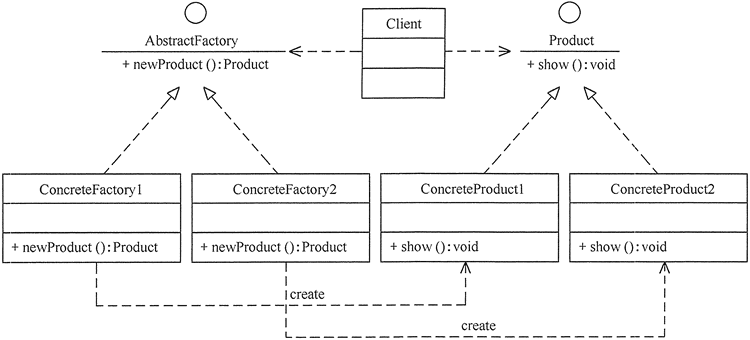
\includegraphics[width=0.8\textwidth]{image/4-1}
	\caption{工厂方法模式的结构图}
\end{figure}
\section{工厂方法——例一}
\begin{lstlisting}
public class AbstractFactoryTest {
	public static void main(String[] args) {
		try {
			Product a;
			AbstractFactory af;
			//从XML文件中读取
			af = (AbstractFactory) ReadXML1.getObject();
			a = af.newProduct();
			a.show();
		} catch (Exception e) {
			System.out.println(e.getMessage());
		}
	}
}

//抽象产品:提供了产品的接口
interface Product {
	public void show();
}

//具体产品1:实现抽象产品中的抽象方法
class ConcreteProduct1 implements Product {
	public void show() {
		System.out.println("具体产品1显示...");
	}
}

//具体产品2:实现抽象产品中的抽象方法
class ConcreteProduct2 implements Product {
	public void show() {
		System.out.println("具体产品2显示...");
	}
}

//抽象工厂:提供了厂品的生成方法
interface AbstractFactory {
	public Product newProduct();
}

//具体工厂1:实现了厂品的生成方法
class ConcreteFactory1 implements AbstractFactory {
	public Product newProduct() {
		System.out.println("具体工厂1生成-->具体产品1...");
		return new ConcreteProduct1();
	}
}

//具体工厂2:实现了厂品的生成方法
class ConcreteFactory2 implements AbstractFactory {
	public Product newProduct() {
		System.out.println("具体工厂2生成-->具体产品2...");
		return new ConcreteProduct2();
	}
}
\end{lstlisting}
\section{模式的扩展}
当需要生成的产品不多且不会增加,一个具体工厂类就可以完成任务时,可删除抽象工厂类。这时工厂方法模式将退化到简单工厂模式。如下图:
\begin{figure}[!h]
	\centering
	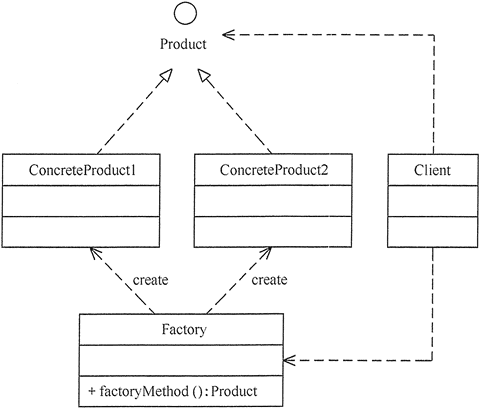
\includegraphics[width=0.6\textwidth]{image/4-2}
	\caption{简单工厂模式的结构图}
\end{figure}
\section{生成实例的三种实现方式}
\begin{enumerate}
	\item 在抽象工厂类中指定createProduct为抽象方法;
	\begin{lstlisting}
abstract class Factory {
	public abstract Product createProduct(String name);
}
	\end{lstlisting}
	\item 使用new实现默认处理;
	\begin{lstlisting}
class Factory {
	public Product createProduct(){
		return new Product(name);
	}
}
	\end{lstlisting}
	\item 在其中抛出异常。
	\begin{lstlisting}
class Factory {
	public Product createProduct(){
		throw new FactoryMethodRuntimeException();
	}
}
	\end{lstlisting}
\end{enumerate}
\section{相关设计模式}
\begin{itemize}
	\item Factory Method是Template Method的经典应用;
	\item 在大多数情况下,Singleton模式用于扮演Creator角色或者ConcreateCreator角色的类。
	\item Composite模式有时可以用于Product角色。
	\item Iterator模式使用iterator生成Iterator实例会使用工厂方法。
\end{itemize}